An einem Datum werden verschiedene Filme zu bestimmten Uhrzeiten gezeigt.
Jeder Film hat einen Titel und einen Regisseur.\\

\noindent
Erstellen Sie das Domänenmodell inklusive Attributen und Multiplizitäten.\\

\noindent
Welches Muster haben Sie wo und wie verwendet?


\section*{Antwort}
S. Abbildung~\ref{fig:film}.

\begin{figure}
    \centering
    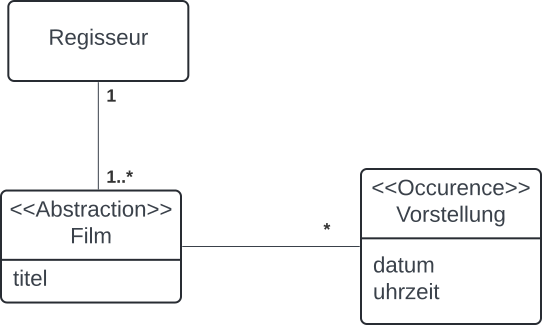
\includegraphics[scale=0.4]{chapters/aufgabe 3/img/film}
    \caption{Domänenmodell für Aufgabe 3. (Quelle: eigene)}
    \label{fig:film}
\end{figure}

\noindent
Anwendung des Musters \textbf{Exemplartyp} für die \code{Film}-\code{Vorstellung}-Assoziation.\\

\noindent
Hierdurch können redundate Informationen in Objekten des Typs \code{Film} vermieden werden: Mehrere Objekte vom Typ \code{Film} hätten sonst identische Attribute wie \code{datum} und \code{uhrzeit}.\\

